\documentclass[twocolumn]{article}
\usepackage[utf8]{inputenc}
\usepackage[english]{babel}
\usepackage{abstract}
\usepackage{booktabs}


\usepackage{graphicx}
\graphicspath{ {latexIMG/} }

\title{Federated Learning where machine learning and data privacy coexists
\\AML Project}
\author{Giuseppe Salvi |
Basiten Bartholom |
Alfredo Baldó Chamorro}
\date{February 2022}

\begin{document}

\maketitle

\section{Abstract}
\section{Introduction} %mandatory
\section{Related Work} %mandatory
\section{Methods} %mandatory describe algorithms
There are various steps in the building of the final algorithm. In this section we will explain the decisions that led us to choose the values for the parameters and our choice for different algorithms implemented. 

Federated learning applied in the real world, would take into account multiple devices with different characteristics (CPU capacity and speed...). The model and algorithm selection was chosen on the basis of a hypothetical implementation on different devices.  

\subsection{Problem setup}
Federated Learning, consist on a client and server side. Considering the CIFAR10 dataset consisting of 60 000 samples, we thought that a number of clients K = 100 would be representing a real world case (averaging 600 images per client). 

Moreover, in order to simulate real world data, we implemented into the code a variability Delta regarding the distribution of the data among clients. The variable added some randomness to the quantity of data that each client would be seeing. 

To add up, the distribution of data was considered to be performed randomly(IS IT TRUE?CONFIRM). The variability Delta introduced was not great, and this was done intentionally. The problem of some client having way bigger amount of images (2-3 times) than others would have been solved with the creation of additional virtual clients and splitting the data among them. 

Finally the number of selected clients C, was chosen based on performance (INSERT TABLE OR GRAPIC). In fact, with a C <0.3 the performance decreased significantly (put some values).
INSERT GRAPHICS BETWEEN DIFFERENT C AND THE CONSOLIDATED MODEL

\subsection{Network}

With that in mind, for the neural network we chose a variation of LeNet5 which has two 5×5, 64-channel convolution layers, each precedes a 2×2 max-pooling layer, followed by two fully-connected layers with 384 and 192 channels respectively and finally a softmax linear classifier (REFERENCE TO PAPER 3 an insert image if possible). 

The implementation of our model takes place in different devices, each having a different computational capacity, we chose a small and simple network in order for the computation to be the quickest possible but also having the capacity to gather information from the client's dataset.

\subsection{Algorithm}
Regarding the server aggregation we chose to go with the Federated Average algorithm (FedAvg). The FedAvg (PUT FORMULA AND REFERENCES) consists on aggregating the weights of the clients according the number of images each client sees, with respect to the total number of images of the dataset.(SPECIFIY MORE AND CORRECT)
The FedAvg algorithm is simple, but useful enough in order to get an acceptable accuracy.

SPEAK ABOUT THE FEDERATED AVERAGE MOMENTUM ALGO

We could say in our report that we considered low difference in the splits because with bigger differences we could have split  the clients in more virtual clients, that has the same result of increasing the number of numclients and selectedclients

\section{Experiments} % mandatory
\subsection{Federated Average}
As baseline model, Federeated Average (FedAvg) algorithm was chosen. In order to get an idea of the performance of the algorithm, a comparison with the centralised model was needed. 

Figure \ref{AccCompFedCent} represents the difference in performance between centralised and federated model. The figure represent a comparison between the two models while changing parameters in the configuration. It's evident and as awaited, that the centralised model has a better performance. The FedAvg does not lead to a good accuracy (hardly reaching 70\%). Still, being a model without any further optimization, the accuracy was thought as acceptable.


\begin{figure}
    \centering
    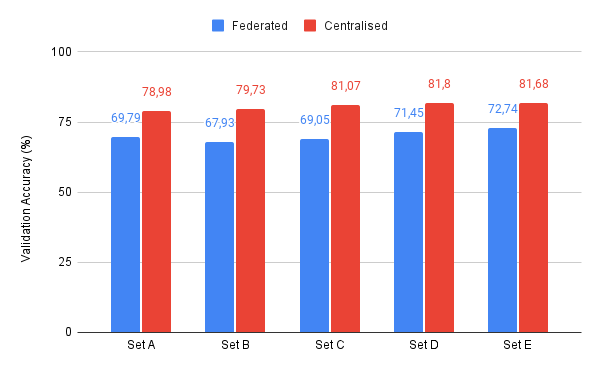
\includegraphics[width=0.5\textwidth,height=.3\textheight]{FedAccuracyComp.png}
    \caption{Accuracy comparison between centralised and federated model}
     \label{AccCompFedCent} 
\end{figure}
\subsection{Group Normalization}
\subsection{Batch Normalization}


\begin{table*}
\centering
\begin{tabular*}{\textwidth}{||c c c c c||} 
  \toprule
 Training loss & Validation Loss & Train Accuracy(\%) & Validation Accuracy (\%) & Batch Normalization \\
  \midrule
  0,6862 & 0,7669 & 75,90 & 73,45 & Yes \\
 \hline
 0,8665 & 0,9963 & 66,05 & 65,49 & No\\
  \bottomrule                             
\end{tabular*}
\label{batchNormComp}
\caption{Performance comparison with batch normalization}
\end{table*}


\subsection{Different data sizes}
In order to simulate different quantity of data that each client is going to have, a variable Delta was implemented in order to add randomness. The experiment was followed by changing the number of groups division of the group normalization layer 1 and 2. The results are represented in figure \ref{AccDiff}, illustrating with different group normalization parameters, the accuracy over the validation set. 

Sticking with figure \ref{AccDiff}, over 8 tests done, three performed better with the Delta variable activated, and one specifically (8-2) outperformed every over scenario with an accuracy of 78,27\%. The accuracies presented in the figure \ref{AccDiff} are very similar between each other, even though with the deactivation of the Delta variable it seems to perform better, as 5/8 tests had greater accuracy than with using Delta.

However, computing the mean of the performances, we get 72,1 \% and 72,8\% for no Delta and Delta respectively. This translates to the fact that even though the Delta variable presented better accuracy, the accuracy achieved with the Delta activated is greater. This results could be explained by the fact that adding some randomness to the data quantities helps the prediction of classes.
DO TWO OR THREE EXPERIMENTS WITH DIFFERENT D

\begin{figure}
    \centering
    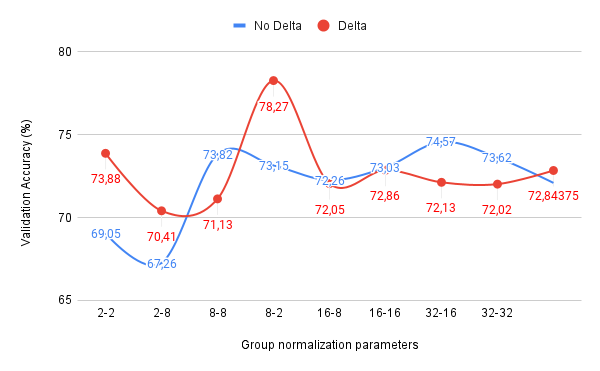
\includegraphics[width=0.5\textwidth,height=.3\textheight]{groupnormalizationDeltaNoDelta.png}
    \caption{Accuracy over validation set with Diff variable activated or not}
     \label{AccDiff} 
\end{figure}

\subsection{Dirichlet distribution}

Regarding implementation, in order to achieve a better understanding of the possible accuracy outcomes, taking into account different data distribution is crucial. In order to simulate that clients get different data distribution, we used the Dirichlet distribution. The parameter Alpha, represents how different the distribution is between clients: with a greater Alpha, the distributions 
would be similar, with smaller Alpha, the distribution between clients differs.

In order to implement it, the implementation was based on data already distributed with different Alpha parameters, taken from (PUT REFERENCE TO GIT REPO).

The results are shown in figure \ref{AccAlpha}. This image clearly illustrates the fact that expanding the difference in the dataset distribution between clients (lower Alpha), as expected, leads to the decrease in accuracy. The accuracy on the training is higher because the smaller the Alpha, the smaller the number of classes each clients gets, hence a perfect prediction is expected. 

Finally, the figure \ref{AccAlpha} states that the group normalization model over-performs the model without normalization (MAYBE WRITE A LITTLE MORE). This results are something expected because they go along with the results gotten in the normalization section. 



\begin{figure}
    \centering
    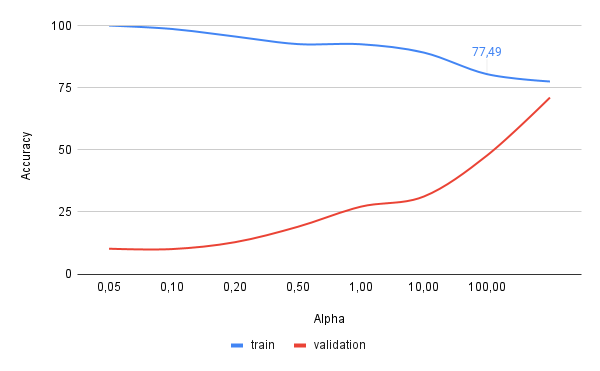
\includegraphics[width=0.5\textwidth,height=.3\textheight]{alphaAccuracy.png}
    \caption{Accuracy over different values of Alpha}
     \label{AccAlpha} 
\end{figure}


\subsection{Federated Average Momentum (additional contribution?)}
MENTION IN THE SETUP THE FEDAV MOMENTUM

\subsection{Conclusion}
SUM UP RESULTS AND 
\subsection{References}


\end{document}
